\documentclass[12pt,aspectratio=169]{beamer}
\usepackage[T2A]{fontenc}
\usepackage[utf8]{inputenc}
\usepackage[russian]{babel}
\usepackage{amsmath,amssymb}
\usepackage{graphicx}
\usepackage{multirow}
\usepackage{booktabs}
\graphicspath{{images/}}%путь к рисункам
\usepackage{svg}  % опция clean удаляет временные файлы
\setsvg{inkscapelatex=true} % глобальная настройка для обработки текста
\svgpath{images/}%путь к рисункам

% Настройка темы оформления
\usetheme{Madrid}
\usecolortheme{default}

% Убираем навигационные символы
\setbeamertemplate{navigation symbols}{}

% Настройка цвета и размера шрифтов
\setbeamerfont{title}{size=\Large}
\setbeamerfont{frametitle}{size=\large}
\setbeamerfont{block title}{size=\normalsize}
\setbeamerfont{footnote}{size=\tiny}

% Информация для титульного слайда
\title[АДМ]{ Разработка модели машинного обучения для распознавания предвестников землетрясений на основе анализа биоэлектрической активности головного мозга животного}
\author[М.Б. Пономарев]{М.Б. Пономарев}
\institute[ИММиКН ЮФУ]{}
\date[2026]{}

\begin{document}
	
	% 1. Титульный слайд
	\begin{frame}
		\titlepage
		\vspace{-1.cm}
		\begin{flushright}
			\small
			Направление подготовки: \\
			01.03.02 Прикладная математика и информатика \\
			%\vspace{0.3cm}
			Научный руководитель:\\ к.т.н., доц. М.Г. Адигеев\\
			ИММиКН им. И.И. Воровича, ЮФУ
		\end{flushright}
	\end{frame}
	
	% 2. Постановка задачи (Цель)
	\begin{frame}{Постановка задачи}
		\begin{block}{Цель работы}
			Разработка и применение метода автоматического обнаружения предсейсмических изменений в динамике парадоксального сна (REM) крыс по данным непрерывной регистрации ЭЭГ.
		\end{block}
		
		\vspace{0.3cm}
		\textbf{Ключевые задачи:}
		\begin{enumerate}
			\item Разработать конвейер преобразования гипнограмм в многомерные временные ряды.
			\item Построить байесовскую модель для поиска точки разладки ($\tau$).
			\item Провести полный перебор и сравнение конфигураций моделей.
			\item Проверить гипотезу о существовании предсейсмического отклика.
			\item Оценить временное окно аномального поведения и оптимальные параметры модели.
		\end{enumerate}
	\end{frame}
	
	% 3. Объект и предмет исследования
	\begin{frame}{Объект и предмет исследования}
		\begin{block}{Объект}
			Биоэлектрическая активность мозга крыс (ЭЭГ) в условиях непрерывного мониторинга на сейсмоактивной территории (Камчатка).
		\end{block}
		
		\vspace{0.3cm}
		\begin{block}{Предмет}
			Статистические закономерности изменения доли REM-сна (REM\%) во временном окне, предшествующем сейсмическому событию.
		\end{block}
		
		\vspace{0.3cm}
		\begin{center}
			\textbf{Гипотеза:} Существует статистически значимое изменение динамики REM\% за несколько суток до землетрясения.
		\end{center}
	\end{frame}
	
	% 4. Экспериментальные данные
	\begin{frame}{Экспериментальные данные}
		\textbf{Выборка:}
		\begin{itemize}
			\item 20 сейсмических событий (2022--2025 гг.) с инструментальной интенсивностью > 2 баллов.
			\item Данные непрерывной регистрации ЭЭГ крыс (особи R1--R4) за 8 дней до и после события.
		\end{itemize}
		
		\vspace{0.3cm}
		\textbf{Предобработка гипнограмм:}
		\begin{enumerate}
			\item Автоматическое стадирование сна (Бодрствование, Медленный сон, REM).
			\item Расчет суточных профилей REM\% методом скользящего окна ($W$, $S$).
			\item Min-Max нормировка для устранения индивидуальных различий.
			\item Разбиение на временные чанки и вычисление описательных статистик (среднее, размах).
		\end{enumerate}
	\end{frame}
	
	% 5. Метод: Байесовская модель точки разладки
	\begin{frame}{Метод: Байесовская модель точки разладки}
		\textbf{Модель:} Поиск единственного момента $\tau$, разделяющего фоновый и аномальный режимы.
		
		\vspace{0.2cm}
		\[
		\mathbf{x}_t \sim 
		\begin{cases}
			p(\mathbf{x}_t \mid \boldsymbol{\theta}_1), & t < \tau \\
			p(\mathbf{x}_t \mid \boldsymbol{\theta}_2), & t \geq \tau
		\end{cases}
		\]
		
		\vspace{0.2cm}
		\textbf{Технические особенности реализации:}
		\begin{itemize}
			\item \textbf{Маргинализация $\tau$:} аналитическое интегрирование дискретного параметра для совместимости с градиентным сэмплером NUTS.
			\item \textbf{Семейства правдоподобия:} Student-t, Lognormal, Beta.
			\item \textbf{Вывод:} Оценка апостериорного распределения $p(\tau \mid \mathcal{D})$ средствами PyMC.
		\end{itemize}
	\end{frame}
	
	% 6. Визуализация 
	\begin{frame}{Визуализация: Байесовская модель точки разладки}
		\begin{center}
			\textbf{Схема модели поиска точки разладки с приорными значениями параметров правдоподобия}
			\vspace{0.05cm}
			
			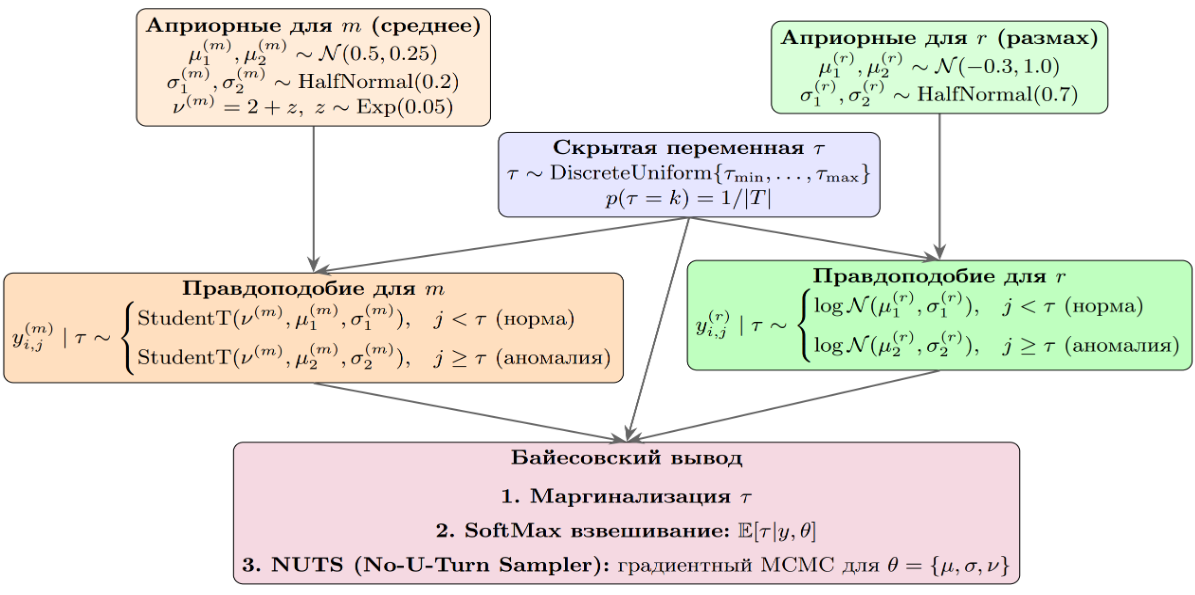
\includegraphics[width=0.7\textwidth]{tau_model.png}
			
			\vspace{0.05cm}
		\end{center}
	\end{frame}
	
	% 6. Программная реализация
	\begin{frame}{Использованные инструменты}
		\begin{columns}[T]
			\begin{column}{0.5\textwidth}
				\textbf{Язык и стек:}
				\begin{itemize}
					\item Python 3.12
					\item PyMC (байесовский вывод)
					\item ArviZ (диагностика MCMC)
					\item NumPy, SciPy, Pandas
				\end{itemize}
			\end{column}
			\begin{column}{0.5\textwidth}
				\textbf{Разработанные модули:}
				\begin{itemize}
					\item \texttt{seismo}: конвейер расчета профилей REM\%.
					\item \texttt{seismic\_pipeline}: полный цикл препроцессинга и моделирования.
				\end{itemize}
			\end{column}
		\end{columns}
		
		\vspace{0.5cm}
		\begin{block}{Ресурсы}
			Вычисления на кластере НИТЦ нейротехнологий ЮФУ (36 физических ядер, JAX-бэкенд). Полный перебор 896 конфигураций выполнен за $\approx 5$ часов.
		\end{block}
		
		\vspace{0.3cm}
		{\tiny Свидетельство о регистрации ПО: «Программа для построения конвейера обработчиков...» № 2026610377.}
	\end{frame}
	
	% 7. Эксперимент: Полный перебор
	\begin{frame}{Дизайн эксперимента: Полный перебор}
		\textbf{Пространство перебора (896 конфигураций):}
		
		\vspace{0.2cm}
		\begin{table}
			\small
			\begin{tabular}{ll}
				\toprule
				\textbf{Фактор} & \textbf{Значения} \\
				\midrule
				Ширина окна ($W$) & 2, 3, 6 часов \\
				Шаг окна ($S$) & 1, 2 часа \\
				Признаки & \texttt{mean}, \texttt{range} \\
				Группировки & \texttt{concat}, \texttt{even}, \texttt{odd} \\
				Правдоподобие & \texttt{student\_t}, \texttt{lognormal}, \texttt{beta} \\
				\bottomrule
			\end{tabular}
		\end{table}
		
		\vspace{0.2cm}
		\textbf{Метрика качества:}
		\begin{itemize}
			\item $\overline{\overline{\mathrm{elpd}}}_{\mathrm{LOO}}$ — дважды нормированная ожидаемая логарифмическая предсказательная плотность (PSIS-LOO).
			\item Диагностика влиятельных наблюдений: Парето $\hat{k}$.
		\end{itemize}
	\end{frame}
	
	% 8. Результат 1: Оптимальная модель
	\begin{frame}{Результат 1: Оптимальная конфигурация}
		\textbf{Лучшая модель значимо превосходит нулевую (без разладки).}
		
		\vspace{0.3cm}
		\begin{block}{Оптимальные параметры}
			\begin{itemize}
				\item \textbf{Признак:} \texttt{concat:mean} (суточная средняя доля REM).
				\item \textbf{Семейство:} \texttt{student\_t} (устойчивость к выбросам).
				\item \textbf{Окно:} $W = 2$ часа (детальный профиль).
			\end{itemize}
		\end{block}
		
		\vspace{0.2cm}
		\begin{itemize}
			\item Признак \texttt{concat:mean} присутствует в \textbf{100\%} топ-5\% моделей и отсутствует в худшем квартиле.
			\item Топ-3 модели статистически неразличимы ($p > 0.05$, парный t-тест), образуя класс эквивалентных решений.
		\end{itemize}
	\end{frame}
	
	% 9. Результат 2: Оценка временного окна
	\begin{frame}{Результат 2: Оценка временного окна}
		\textbf{Гипотеза подтверждена: обнаружен устойчивый сигнал.}
		
		\vspace{0.3cm}
		\begin{center}
			\large
			$\mathbb{E}[\tau] \approx \mathbf{6.6 \pm 0.4}$ \textbf{дней до толчка}
		\end{center}
		
		\vspace{0.3cm}
		\textbf{Свойства оценки:}
		\begin{itemize}
			\item Апостериорное распределение $\tau$ сконцентрировано в диапазоне 6--7 дней.
			\item Оценка устойчива: разброс среднего $\mathbb{E}[\tau]$ между квартилями ELPD менее 0.2 суток.
			\item Высокая робастность: в топ-10 моделях отсутствуют влиятельные события ($\hat{k} < 0.7$).
		\end{itemize}
	\end{frame}
	
	% 10. Результат 3: Анализ признаков
	\begin{frame}{Результат 3: Роль признаков и робастность}
		\textbf{Компромисс точности и качества:}
		\begin{itemize}
			\item Признак \texttt{range} (размах) \textbf{сужает} распределение $\tau$ в $1.3$--$1.9$ раза.
			\item \textbf{НО}: добавление \texttt{range} значимо \textbf{снижает} общую предсказательную силу модели (ELPD).
		\end{itemize}
		
		\vspace{0.3cm}
		\textbf{Анализ влиятельных событий:}
		\begin{itemize}
			\item В топ-10 моделях нет событий с $\hat{k} \geq 0.7$.
			\item Это подтверждает, что выводы не держатся на единичных выбросах, а отражают общую для выборки закономерность.
		\end{itemize}
		
		\vspace{0.3cm}
		\textbf{Вывод:} Для предсказания лучше всего использовать только суточное среднее REM\%.
	\end{frame}
	
% 11. Визуализация 
\begin{frame}{Визуализация: Апостериорное распределение $\tau$}
	\begin{center}
		\textbf{График  $\mathbf{Q}_2(\tau)$ по всем моделям.}
		\vspace{0.05cm}
		
		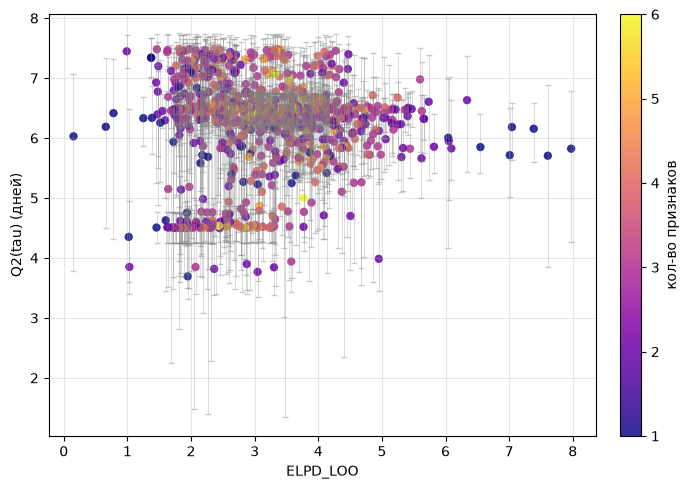
\includegraphics[width=0.5\textwidth]{q2_tau.png}
		%\caption{ Усы - $\mathbf{Q}_1(\tau)$ и $\mathbf{Q}_3(\tau)$, цвет точки указывает на количество используемых моделью признаков.}
		%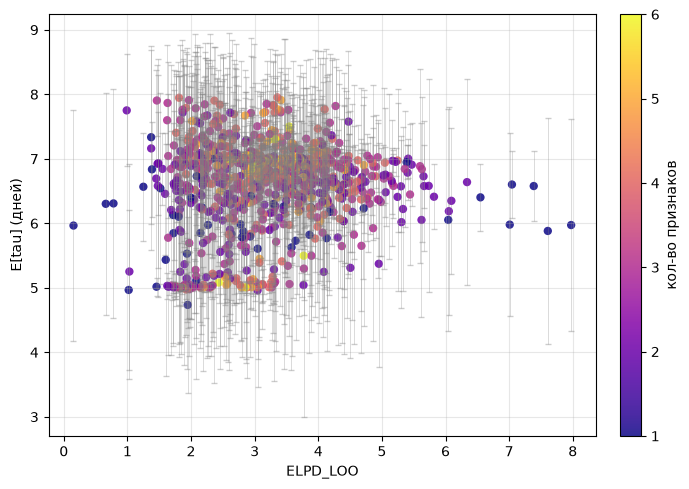
\includegraphics[width=0.5\textwidth]{e_tau.png}
		
		\vspace{0.05cm}
		{\small Подавляющее большинство моделей указывает на точку разладки между 6 и 7 днем.}
		\vspace{0.1cm}
		{\small Модели с разладкой на 1--3 день отсутствуют.}
	\end{center}
\end{frame}
	
	% 12. Визуализация 
	\begin{frame}{Визуализация: Распределение ELPD}
		\begin{center}
			\textbf{Q-Q график распределения ELPD}
			\vspace{0.05cm}
			
			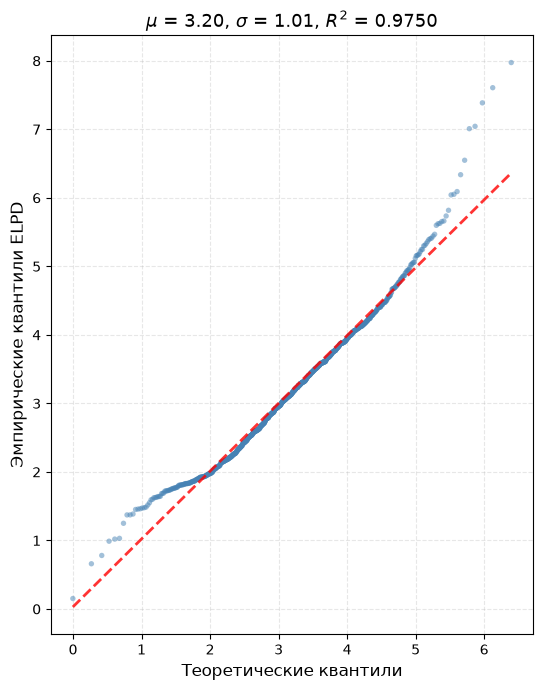
\includegraphics[width=0.4\textwidth, height=5.5cm]{qq_elpd.png}
			
			\vspace{0.05cm}
			{\small Распределение ELPD близко к нормальному, но имеет выраженные хвосты \linebreak (класс моделей-лидеров).}
		\end{center}
	\end{frame}
	
	% 13. Итоговые результаты
	\begin{frame}{Основные результаты работы}
		\textbf{В ходе исследования:}
		\begin{enumerate}
			\item Разработан и реализован конвейер предобработки гипнограмм и вычисления признаков REM-сна (свидетельство о гос. регистрации ПО).
			\item Построена байесовская changepoint-модель с маргинализацией $\tau$, позволяющая эффективно оценивать момент смены режима.
			\item Проведен полный перебор \textbf{896 конфигураций} и на основе метрики ELPD определена оптимальная структура модели.
			\item \textbf{Подтверждена гипотеза} о существовании статистически значимого изменения REM\% перед землетрясением.
			\item Установлено, что аномалия проявляется в среднем в окрестности \textbf{2 -- 3 дней} до и после сейсмического события.
		\end{enumerate}
	\end{frame}
	
	% 14. Слайд с результатами
	\begin{frame}{Результаты}
		\begin{center}
			\large \textbf{Полученные результаты}
		\end{center}
		
		\vspace{0.3cm}
		\begin{enumerate}
			\item \textbf{Метод:} Разработан метод поиска предсейсмических аномалий в динамике REM-сна на основе байесовского вывода.
			\item \textbf{Модель:} Оптимальная модель использует \texttt{concat:mean} и \texttt{Student-t} правдоподобие при ширине окна 2 ч.
			\item \textbf{Окно:} Аномальные изменения происходят в интервале \textbf{2--3 дней} до и после толчка.
			\item \textbf{Робастность:} Выводы устойчивы к выбору метрик и исключению влиятельных событий.
		\end{enumerate}
	\end{frame}
	
\end{document}